\section{Considerações Iniciais}

Refatorações são técnicas bem conhecidas que auxiliam desenvolvedores durante a reformulação de um determinado sistema com o objetivo de melhorar atributos internos e ainda possuem a preocupação de preservar o comportamento original do sistema. Como já salientado no Capítulo~\ref{chapter:fundamentacao_teorica} Seção~\ref{sec:refatoracao}, refatorações são geralmente utilizadas durante o processo de engenharia reversa, cujo o objetivo é mudar a estrutura de um determinado sistema para resolver os problemas estruturais identificados anteriormente. Em uma linha de pesquisa paralela, como destacado no Capítulo~\ref{chapter:adm_kdm}, existe a ADM que consiste em nova geração de processos para auxiliar e padronizar as atividades da engenharia reversa; utilizando apenas modelos ao invés de código-fonte como os principais artefatos durante o processo de modernização. Embora o OMG forneça conceitos gerais para a condução de modernização dirigida à modelos por meio da ADM, ele não fornece instruções sobre como criar ou aplicar refatorações em seus metamodelos, ou seja, no metamodelo KDM. Ainda que a ADM tenha solicitado um \textit{call for proposal} denominado ADM \textit{Refactoring}\footnote{Até o momento da escrita desta Tese a padronização denominada ADM \textit{Refactoring} estava em estágio de discussão. Assim, uma das principais contribuições deste capítulo é auxiliar na criação e adaptação de soluções de refatorações para o metamodelo KDM.} para propor e desenvolver soluções que auxiliam o modernizador durante as atividades de refatorações de sistemas com a utilização do metamodelo KDM até o momento existe uma carência de soluções padronizadas e apoios ferramentais. A ausência de instruções de como criar e adaptar refatorações já existentes para o metamodelo KDM faz com que desenvolvedores/modernizadores criem suas próprias soluções. Usualmente tais soluções tendem a se tornarem proprietárias o que pode dificultar o reuso, diminuindo assim a interoperabilidade, um dos principais objetivos da ADM.

O conjunto de refatoração mais conhecido e útil é o catálogo proposto por~\citeonline{Fowler1999}. Porém, esse catálogo foi proposto primeiramente para ser utilizado em código-fonte, não em modelos, como a UML e KDM. Embora~\citeonline{Fowler1999} tenha criado um catálogo de refatorações para ser utilizado em código-fonte, mais de 60\% das refatorações (44 de 72) são ilustradas e explicadas utilizando modelos. Esta observação levanta a questão se refatorações \aspas{tradicionais}, ou seja, aquelas aplicadas em código-fonte, podem ser adaptadas e criadas para modelos como o KDM. ~\citeonline{Zhang_2005, Boger_2003} afirmam que algumas refatorações, por exemplo, \texttt{Extract Method}, são mais naturais quando executadas diretamente no código-fonte. Outras refatorações, como, \texttt{Rename Class}, \texttt{Pull Up Method}, \texttt{Push Down Method}, etc, podem ser aplicadas tanto em código-fonte quando em modelos; já as refatorações que lidam com herança, tais como \texttt{Extract Class}, \texttt{Extract Interface}, \texttt{Replace Inheritance with Delegation}, são mais intuitivas quando aplicadas diretamente em nível de modelo. 

Embora a refatoração no contexto de modelo tenha alcançado bastante reconhecimento e aceitação na literatura~\cite{Moghadam_2012, Maneerat_2011, Fourati_2011, Einarsson_2012, Steimann_2015, Akiyama_2011, Jensen_2010, Arendt_2012, Millan_2009, Tom_2008_2008}, ainda se faz necessário pesquisas nessa área~\cite{durelli_systematic_mapping, revisao_sistematica_uml_refactoring}. Como já salientado até esse momento existe uma ausência de catálogos de refatoração e ferramentas que auxiliem os modernizadores de software à aplicar refatorações de forma consistente para instâncias do metamodelo KDM. Dessa forma, os engenheiros precisam desenvolver suas próprias refatorações, catálogos e apoios ferramentais para refatorar diversos sistemas. Como consequência, essas soluções tornam-se difíceis de serem reutilizadas diminuindo assim a interoperabilidade entre as ferramentas de modernização. 

Diante desse contexto, neste capítulo é identificado e descrito um conjunto de atividades pertinentes para auxiliar a criação e adaptação de refatorações para serem aplicadas em instâncias do metamodelo KDM. As refatorações apresentadas e adaptadas neste capítulo são baseadas no catálogo de refatoração do~\citeonline{Fowler1999}. O intuito dessas refatorações é facilitar a condução da modernização de um determinado sistema legado representado como uma instância do metamodelo KDM~\cite{durelli_catalogo, durelli_VEM_ferramenta}. Ainda neste capítulo é apresentado um mapeamento entre os conceitos do paradigma orientado a objetos para o metamodelo KDM, assim, engenheiros de modernização podem de forma mais fácil adaptar novas refatorações para o metamodelo KDM. Nota-se que esse capítulo é uma extensão do seguinte artigo: \textit{Towards a Refactoring Catalogue for Knowledge Discovery Metamodel}~\cite{durelli_catalogo}.

Com o intuito de apresentar e facilitar o entendimento das refatorações adaptado para o KDM de uma maneira mais prática, neste capítulo apenas algumas refatorações são apresentadas. É importante destacar que as refatorações são implementadas com o uso da ATL~\cite{Allilaire_06, Jouault_2005, Jouault_2008} e as pre- e pós-condições são implementadas utilizando OCL. ATL e OCL foram escolhidas nesta Tese pois ambas são linguagens bem conhecidas e amplamente utilizadas na literatura. Porém, ressalta-se que as refatorações, bem como as pré- e pós-condições podem ser adaptadas com o uso de outras tecnologias, como, por exemplo, \textit{Query/View/Transformation}~\cite{QVT:OMG}, EMF Henshin~\cite{EMF_Henshin}, SmartQVT~\cite{SmartQVT}, ModelMorf~\cite{ModelMorf}, Kermeta~\cite{kermeta}, \textit{Epsilon Transformation Language}~\cite{ETL_eclipse}, OpenArchitectureWare~\cite{OpenArchitectureWare}, VIATRA~\cite{viatra}, AndroMDA~\cite{andromda} e Fujaba \textit{transformations}~\cite{fujaba}.

As demais seções desta capítulo estão organizadas da seguinte forma:\change{terminar aqui. Deve colocar todas as seções bem escritas.}

\section{Estrategia para Adaptar Refatorações o metamodelo KDM}

Refatorações dirigidas à modelos são transformações especiais que são aplicadas em modelos para melhorar a estrutura de um determinado modelo e ainda preservar suas características internas. Refatorações dirigidas à modelos é uma área relativamente nova quando comparada com refatorações tradicionais, ou seja, aquelas aplicadas em código-fonte. Com base em informações obtidas das refatorações tradicionais e de abordagens dirigidas à modelos, foi possível identificar uma lista de atividades distintas que são essenciais para a definição e adaptação de refatorações para o contexto da ADM e KDM. Essa lista é apresentada a seguir:

\begin{itemize}
\item Elementos Estruturais: Mapear os conceitos de POO para o metamodelo KDM.
Aqui é necessário identificar os elementos do POO que são correspondentes no metamodelo KDM;
\item Linguagem de Transformação de Modelo: Utilizar uma linguagem de transformação para a definição e adaptação do mecanismo da refatoração. Elementos Estruturais juntamente com a Linguagem de Transformação de Modelo formam o sistema de transformação;
\item Linguagem de Restrições: Utilizar uma linguagem de restrição para garantir a preservação de comportamento ao aplicação uma refatoração. Instâncias do metamodelo KDM são entidades não executáveis, assim, se faz necessário a utilização de linguagens de restrições para garantir a correta execução da refatoração antes e depois de sua aplicação;
\item Refatorações: Selecionar um conjunto de refatorações que podem ser adaptadas para o metamodelo KDM;
\item \textit{Template}: Definir um modelo de como as refatorações são informalmente e formalmente apresentadas;
\item Apoio computacional: Definir um ambiente computacional para auxiliar o engenheiro a aplicar a refatoração. A refatoração pode ou não ser aplicada sem a intervenção de um usuário;
\item Gerenciamento de consistência: Refatorar uma instância de um determinado modelo pode fazer com que o mesmo se torce inconsistente. Para preservar consistência entre as visões da instância do modelo abordagens de preservação de consistência precisam ser adotadas.
\end{itemize}

Nas subseções a seguir tais atividades são apresentadas e detalhadas com maiores detalhes. Os dois últimos itens da lista, apoio computacional e gerenciamento de consistência, são apresentados em outros capítulos. A ferramenta KDM-RE é apresentada no Capítulo~\ref{chapter:ferramenta_kdm_re} e a abordagem KDM-SInc é apresentada no Capítulo~\ref{chapter:Abordagem_de_sincronizacao}.

\subsection{Elementos Estruturais}\label{sec:mapeamento_POO_e_KDM}
Nesta atividade o objetivo é traduzir os conceitos do POO para o metamodelo KDM, ou seja, identificar os elementos estruturais do POO para o metamodelo KDM. De acordo com \citeonline{Zhang_2005, Boger_2003} um dos maiores desafios quando necessita-se realizar adaptar refatorações para um determinado metamodelo é saber quais são as metaclasses corretas que representam determinadas construções/declarações de um determinado paradigma de programação, no contexto desse capítulo, POO. Em outras palavras, é importante identificar se a metaclasse escolhida para fazer a refatoração representa realmente o elemento e o conceito do POO. Dessa forma, antes de realizar a adaptação de qualquer refatoração para o metamodelo KDM, deve-se primeiramente identificar as metaclasses do KDM que têm características similares aos conceitos do POO, bem como instruções comumente utilizadas em todas as linguagens de programação, tais como, ramificações, iterações, etc. 

Consequentemente, foi necessário fazer um mapeamento entre os conceitos do POO e o metamodelo KDM. Esse mapeamento pode ser visto na Tabela~\ref{tab:mapemanetoEntreOOPeKDM}. Essa tabela de mapeamento identifica metaclasses do KDM que possuem características similares aos conceitos do POO, uma vez que as refatorações propostas por~\citeonline{Fowler1999} e adaptadas aqui, são especificas e definidas para o POO, assim, tal tabela se faz necessário; com base nessa Tabela~\ref{tab:mapemanetoEntreOOPeKDM} é argumentado que modernizadores podem criar outras refatorações seguindo esse mapeamento, assim, qualquer exemplo de refatoração pode ser facilmente adaptada para o metamodelo KDM. 

Esta Tabela~\ref{tab:mapemanetoEntreOOPeKDM} contêm três colunas, \aspas{Elemento do Código-fonte}, \aspas{Pacote::metaclasse do KDM} e \aspas{Descrição}. A primeira coluna informa a construção da linguagem de programação (\textit{statement})e/ou o conceito e do POO (pacote, classe, interface, etc), respectivamente. Em seguida a coluna \aspas{Pacote::metaclasse do KDM} apresenta a metaclasse responsável por mapear a construção e/ou o conceito do POO. Note que essa coluna segue o formato \aspas{Package::Meta-class}. A ultima coluna, \aspas{Descrição}, contêm informações sobre a metaclasse, por exemplo, essa coluna contêm importantes meta-atributos e meta-associações que são utilizadas durante uma refatoração.


\begin{center}
\begin{longtable}{ | m{1.9cm} | m{3.57cm}| m{9.3cm} | } 
\caption{Mapeamento do POO e Código-Fonte para KDM.\label{tab:mapemanetoEntreOOPeKDM}}\\
\hline
Elemento do Código-Fonte & Pacote::metaclasse do KDM & Descrição \\ 
\hline
Pacote & code::Package & A metaclasse \texttt{Package} é um contêiner para elementos de programa, como classes e interfaces. Essa metaclasse contêm um principal meta-atributo, \texttt{name}, que especifica o nome do pacote. Além disso, esta metaclasse contêm uma principal meta-associação \texttt{codeElement:AbstractCodeElement[0..*]} onde, pacotes, classes e interfaces podem ser incluídos. \\ 
\hline
Classe & code::ClassUnit & A metaclasse \texttt{ClassUnit} possui dois principais meta-atributos,  \texttt{name:String} e \texttt{isAbstract:boolean}. O primeiro é utilizado para especificar o nome da classe, o segundo é utilizado para informar se a classe é ou não abstrata. Além disso, essa metaclasse possui três meta-associações: \texttt{attribute:Attribute[0..*]}, \texttt{codeRelation:KDMRelationship[0..*]} e  \texttt{codeElement:AbstractCodeElement[0..*]}. \texttt{attribute} é utilizado para especificar a  visibilidade da classe, ou seja, \textit{public}, \textit{private}, ou \textit{protected}. \texttt{codeRelation} agrupa todos os relacionamentos que uma determinada classe contêm, por exemplo, heranças e associações. \texttt{codeElement} agrupa qualquer metaclasse cujo tipo é uma concretização de \texttt{AbstractCodeElement}, como: \texttt{StorableUnit}, \texttt{MethodUnit}, \texttt{MemberUnit}, etc. \\ 
\hline
Interface & code::InterfaceUnit & A metaclasse \texttt{InterfaceUnit} possui características similares a metaclasse \texttt{ClassUnit}, porém, não tem o meta-atributo \texttt{isAbstract}, uma vez que todas as interfaces são abstratas por padrão. \\ 
\hline
Atributo & code::StorableUnit & A metaclasse \texttt{StorableUnit} possui dois principais meta-atributos: \texttt{name:String} e \texttt{kind:StorableKind}. Similarmente, esse metaclasse possui duas principais meta-relacionamentos: \texttt{attribute:Attribute[..*]} e \texttt{type:DataType[1]}. \texttt{name} é utilizado para especificar o nome do atributo. \texttt{kind} é uma enumeração utilizada para especificar propriedades do atributo, ou seja, informar se o mesmo é local, global, estático, etc. \texttt{attribute} é utilizado para definir o escopo do atributo, \textit{public}, \textit{private}, ou \textit{protected}. E \texttt{type} é utilizado para definir o tipo do atributo.  \\ 
\hline
Método & code::MethodUnit & A metaclasse \texttt{MethodUnit} possui dois principais meta-atributos: \texttt{name:String} e \texttt{kind:MethodKind}. \texttt{name} é utilizado para especificar o nome do método. \texttt{kind} é uma enumeração utilizada para especificar propriedades do método, ou seja, informar se o método é \textit{construtor}, \textit{destructor}, \textit{virtual}, \textit{abstract}, etc. Similarmente, esse metaclasse possui dois principais meta-relacionamentos: \texttt{attribute:Attribute[..*]}, \texttt{codeElement:AbstractCodeElement[0..*]}. \texttt{attribute} é utilizado para definir o escopo do método - informar se o mesmo é \textit{public}, \textit{private}, ou \textit{protected}. E \texttt{codeElement} é utilizado para agrupar declarações internas do método, ou seja, assinatura do método, bloco do método, etc.\\ 
\hline
Assinatura do Método & code::Signature & A metaclasse \texttt{Signature} possui um principal meta-atributo, \texttt{name:String}, o qual é utilizado para especificar o nome do método. Além disso, essa metaclasse contêm um principal meta-relacionamento denominado \texttt{parameterUnit:ParameterUnit[..*]} que é utilizado para especificar os parâmetros que o método contêm.\\ 
\hline
Bloco do Método & action::BlockUnit & A metaclasse \texttt{BlockUnit} representa blocos lógicos e físicos relacionados, por exemplo, blocos de instruções \textit{if}, \textit{for}, \textit{while}, etc. Possui um meta-relacionamento denominado \texttt{codeElement:AbstractCodeElement[0..*]} que é utilizado para agrupar qualquer instruções lógicas ou físicas.\\ 
\hline
Parâmetro & code::ParameterUnit & A metaclasse \texttt{ParameterUnit} pode representar o nome, tipo e a posição dos parâmetros em uma assinatura de método. além de permitir o tipo de parâmetro (valor ou referência). Essa metaclasse contêm dois principais meta-atributos: \texttt{name:String} e \texttt{kind:ParameterKind}. O primeiro meta-atributo representa o nome do parâmetro, o segundo meta-atributo é uma enumeração para especificar o tipo de parâmetro (valor ou referência). Além disso, \texttt{ParameterUnit} contêm o meta-relacionamento \texttt{type:DataType[1]} para especificar o tipo do parâmetro, esse tipo pode ser tipos primitivos ou outros tipos.\\ 
\hline
Associação & code::HasType & A metaclasse \texttt{HasType} representa relação semântica entre um elemento de dados e seu tipo. Essa meta-calsse contêm duas principais meta-relacionamentos: \texttt{from:CodeItem} e \texttt{to:DataType}.\\ 
\hline
Herança \texttt{extends} & code::Extends & A metaclasse \texttt{Extends} representa relação semântica de herança entre duas \texttt{ClassUnits} ou duas \texttt{InterfaceUnits}. Essa relação semântica é representada por dois meta-relacionamentos: \texttt{from:DataType} e \texttt{to:DataType}.\\ 
\hline
Herança \texttt{implements} & code::Implements & A metaclasse \texttt{Implements} representa relação semântica de herança entre uma \texttt{ClassUnit} e uma \texttt{InterfaceUnit}. Similarmente a metaclasse \texttt{Extends} a relação semântica é representada por dois meta-relacionamentos: \texttt{from:DataType} e \texttt{to:DataType}.\\ 
\hline
\textit{if}, \textit{for}, \textit{while}, etc & action::ActionElement & \texttt{ActionElement} representa instruções e declarações de uma determinada linguagem de programação, ou seja, pode ser utilizada para representar ramificações, iterações, etc. \texttt{ActionElement} possui um principal meta-atributo denominado \texttt{kind:String} que representa qual o tipo instrução que a metaclasse esta representando. Essa metaclasse possui dois meta-relacionamentos \texttt{codeElement:AbstractCodeElement[0..*]} e \texttt{actionRelation:ActionRelationship[0..*]}.\\ 
\hline
\end{longtable}
\end{center}

Na Tabela~\ref{tab:mapemanetoEntreOOPeKDM} é possível ver a relação existente entre os conceitos do POO, bem como algumas instruções de linguagens de programação e o metamodelo KDM. Para atender aos objetivos deste trabalho essa tabela de mapeamento mostra apenas os principais elementos que são utilizados no catálogo de refatoração adaptado para o KDM, uma vez que seria inviável mapear todas as noventa metaclasses do metamodelo KDM.

É importante observar nessa tabela de mapeamento que algumas metaclasses podem ser diretamente mapeadas, tal como, classes, interfaces, atributos, métodos, etc. Essas metaclasses possuem o mesmo objetivo e características dentro do contexto do POO e linguagens de programação. Entretanto, como o KDM tem como objetivo ser um modelo independente de plataforma, ou seja, tem como intuito representar de forma genérica todas as abstrações e paradigmas de programação, algumas construções de programação não possuem uma metaclasse particular. Por exemplo, iterações e ramificações em KDM são representadas utilizando a mesma metaclasse, \texttt{ActionElement}. Esse mapeamento ocorre pois o KDM define uma metaclasse genérica para especificar ramificações e iterações para preservar a independência de plataforma; seria inviável para o metamodelo definir específicas metaclasses para representar ramificações e iterações uma vez que cada linguagem de programação possui um determinada particularidade. Para que o mapeamento fique o mais genérico e independente de plataforma possível a metaclasse \texttt{ActionElement} utiliza o meta-atributo \texttt{kind}, o qual contêm os seguintes valores: \textit{variable declaration}, \textit{if}, \textit{for}, \textit{while}, etc.

\subsection{Linguagem de Transformação De Modelo}

Na literatura é possível identificar um conjunto de técnicas e linguagens específicas para auxiliar a condução e especificação de transformação de modelos~\cite{Biehl_2010, Mens_2006, Allilaire_06}. A seguir é apresentado as duas abordagens mais utilizadas na literatura para a elaboração e condução de refatorações para modelos: (\textit{i}) Abordagem de Manipulação Direta: Essa abordagem utiliza linguagens de programação tradicional para a aplicação das refatorações. Ferramentas que utilizam essa abordagem utilizam linguagens como Java, C, C++ etc~\cite{Bruneliere_2014}. Usualmente tais linguagens proporcionam uma infraestrutura mínima para organizar as transformações. Algumas características de suma importância para refatorações de modelo como, regras de transformações, preservação de comportamento são, usualmente criadas pelo engenheiro, uma vez que tais linguagens não possuem API para lidar com tais características. Dessa forma, refatorações que utilizam essa abordagem tendem a ser dependente de plataformas, afetando assim a reusabilidade das refatorações; e (\textit{ii}) Abordagem de Transformação Genérica: Essa abordagem utiliza linguagens desenvolvidas especialmente para realizar transformações em modelos, tais como ATL, QVT, Kermeta, etc. Usualmente, tais abordagens são conhecidas como endógenas e são implementadas utilizando técnicas de reescrita de grafo, ou como também é conhecida transformação de grafo (ver Capítulo~\ref{chapter:fundamentacao_teorica} Seção~\ref{sec:transformacoes_de_modelos}). Diferentemente a abordagem anterior, essa abordagem facilita o reuso de refatorações, uma vez que tais abordagens foram criadas para serem independentes. Por exemplo, utilizando essa abordagem o engenheiro pode criar um conjunto de regras de refatorações por meio de linguagens de transformações genéricas, assim, tais refatorações podem ser invocadas utilizando qualquer linguagem de programação. O engenheiro poderia escrever um código em Java que iria ter como entrada uma instância do metamodelo KDM para ser refatorado, a reforação a ser aplicada nessa instância e um conjunto de parâmetros para realizar a refatoração na instância do metamodelo KDM.

Nesta Tese, a segunda abordagem é utilizada, ou seja, a abordagem de transformação genérica foi escolhida para auxiliar na definição das refatorações. Mais especificamente a linguagem de transformação ATL~\cite{ATL_eclipse,Jouault_2008} foi escolhida para definir e aplicar refatorações no metamodelo KDM. ATL foi escolhida como linguagem de transformação considerando vários aspectos. Essa linguagem está integrada na plataforma Eclipse, o que fornece uma série de recursos padrões para o desenvolvimento (\textit{syntax highlighting} e \textit{debugger}). ATL é parte do projeto \textit{Model-To-Model} e possui um grupo de discussão ativo, constantemente atualizado, vários exemplos e diversos estudos de casos aplicados até mesmo na indústria utilizam tais linguagens. Além disso, com a utilização da ATL as refatorações definidas podem ser facilmente reutilizadas e compartilhadas em nível de metadados.

\subsection{Linguagem de Restrições}

Nesta atividade as formas de especificar as restrições foram identificadas para definir as pré- e pós-condições de uma determinada refatoração. Usualmente antes e após a aplicação de uma determinada refatoração algumas restrições precisam ser satisfeitas. Tais restrições usualmente são úteis para verificar se os parâmetros necessários para executar a refatoração foi completamente e corretamente informando, bem como verificar se a refatoração foi aplicada de forma totalmente correta. No contexto de modelos, tais restrições são especificadas utilizando linguagem como OCL. Tais restrições no contexto de refatorações são conhecidas como pré- e pós-condições. Utilizando essa linguagem, é possível verificar, por exemplo, se todos os parâmetros obrigatórios para executar o mecanismo da refatoração foram especificados pelo modernizador. Além disso, essas condições são importantes para assegurar que a refatoração será aplicada de forma correta e ainda irá preservar a semântica da instância do meta-modelo, como por exemplo, preservar comportamentos, sincronização, etc. 

Dessa forma, cada refatoração definida nesta Tese está associada com uma pré- e pós-condição definida em OCL. OCL foi escolhida pois a mesma é uma linguagem padronizada pela OMG e também possui suporte na plataforma Eclipse


\subsection{Refatoração para o Metamodelo KDM}

Nesta seção algumas das refatorações propostas por~\citeonline{Fowler1999} são escolhidas para serem adaptadas para o contexto do metamodelo KDM. Escolhe-se as refatorações definidas por~\citeonline{Fowler1999} uma vez que tais refatorações são bem conhecidas, básicas e de baixa granularidade. É importante salientar que as refatorações adaptadas seguem o mesmo \textit{template} definidos em~\citeonline{Fowler1999}, porém, os nomes de algumas refatorações foram alteradas para indicar o metamodelo KDM como seu novo domínio de aplicação, por exemplo, \texttt{MoveMethod} torna-se \texttt{MoveMethodUnit} e \texttt{MoveAttribute} torna-se \texttt{MoveStorableUnit}, etc. 

No contexto desta Tese todas as refatorações são transformações que são realizadas em uma instância do metamodelo KDM. Assim, todas as refatorações podem ser agrupadas em nível de sua granularidade. As granularidades podem ser definidas em dois níveis de operações: (\textit{i}) operações atômicas e (\textit{ii}) operações compostas.As granularidades definidas como operações atômicas podem ser especificadas por meio de operações primitivas que são executadas na instância do metamodelo KDM. Tais operações primitivas são listadas a seguir:

\begin{itemize}
\item \texttt{add}: qualquer operação que adicione uma instância de uma metaclasse do metamodelo KDM (ver Tabela~\ref{tab:mapemanetoEntreOOPeKDM});
\item \texttt{delete}: qualquer operação que remove uma instância de uma metaclasse do metamodelo KDM (ver Tabela~\ref{tab:mapemanetoEntreOOPeKDM});
\item \texttt{change}: qualquer operação que altere um valor de um meta-atributo de uma metaclasse do metamodelo KDM (ver Tabela~\ref{tab:mapemanetoEntreOOPeKDM}).
\end{itemize}

As refatorações de granularidade compostas consistem em uma combinação de operações atômicas, por exemplo, a operação \texttt{move} consiste em uma combinação das operações atômicas \texttt{add} e \texttt{delete}.


Com o intuito de facilitar a visualização, formalização e entendimento das refatorações adaptadas para o metamodelo KDM, todas as refatorações consistem de duas principais especificações~\cite{staron2004implementing} - uma especificação informal e uma especificação formal. Na especificação informal a ideologia básica por trás da reforação é expressada, usualmente essa ideologia é definida por meio de linguagem natural. A segunda especificação, a especificação formal é responsável por representar as pré- e pós-condições, bem como a transformação/refatoração propriamente dita em linguagens executáveis, ou seja, OCL e ATL são utilizadas na especificação formal, respectivamente. Ambas especificações são úteis para o engenheiro de modernização - a especificação informal é utilizada para facilitar a compreensão e o propósito da refatoração, enquanto que a especificação formal facilita a implementação da refatoração. Além disso, a especificação formal é de extrema importância para facilitar a automação das refatorações. Maiores detalhes sobre essas especificações são apresentados na Subseção~\ref{sec:template_refatoracao}.

Consequentemente, pode-se definir que no contexto desta Tese cada refatoração consiste em uma transformação de modelos que possui pre- e pós-condições particulares que devem ser satisfeitas antes e depois da transformação/refatoração ser executada. Por exemplo, a refatoração \texttt{Remove ClassUnit} têm como pré-condição que uma determinada instância de \texttt{ClassUnit} deve existir na instância do KDM a ser refatoração e não ser referenciada. Nota-se que a definição de refatoração no contexto desta Tese engloba transformações que preservam o comportamento no contexto de modelos. A Definição~\ref{def:refatoracao} formaliza refatorações para o contexto desta Tese:


\begin{definicao}\label{def:refatoracao}
    \textit{Uma refatoração é uma tripla ordenada $R = (pre, T, P)$ onde \textbf{pre} é uma asserção (ou seja, pré-condição) que deve ser verdade em uma determinada instância \textbf{R} do metamodelo KDM, \textbf{T} consiste na transformação do modelo \textbf{R}, e \textbf{P} é a pós-condição a ser aplicada após \textbf{T} ser executada.}
\end{definicao}


\subsection{\textit{Template} de Definição de Refatoração para o metamodelo KDM}\label{sec:template_refatoracao}

Dado a Definição~\ref{def:refatoracao} de refatoração no contexto desta Tese é importante apresentar como cada refatoração é especificada. Como já salientado, as refatorações são definidas utilizando duas especificações, informal e formal. Assim, cada refatoração está especificada utilizando o seguinte \textit{template}:

\begin{enumerate}
	\item Especificação Informal:
		\begin{enumerate}
			\item Nome: o nome da refatoração;
			\item Definição: uma lista contendo os parâmetros utilizados na refatoração - após a definição dos parâmetros, eles são utilizados e referenciados dentro das especificações formal e informal por meio de \{...\};
			\item Objetivo: o objetivo da refatoração;
			\item Descrição (opcional): uma pequena explicação da refatoração;
			\item Pré-condição: uma lista de asserção que tem que ser verdade antes de realizar a refatoração;
			\item Pós-condição: uma lista de asserção que tem que ser verdade após a realização da refatoração;
			\item Mecanismo: uma mecanismo de transformação descrevendo todos os passos da refatoração, seguido de uma imagem ilustrando o antes e depois da aplicação da refatoração;
			\item Algoritmo: um algoritmo que descreve a refatoração.
		\end{enumerate}
	\item Especificação Formal:
		\begin{enumerate}
			\item Pré-condição: a pré-condição expressa em OCL;
			\item Algoritmo: a refatoração (\textit{model transformation}) definida em ATL;
			\item Pós-condição: a pós-condição expressa em OCL.
		\end{enumerate}
\end{enumerate}


\section{Catálogo de Refatoração para o metamodelo KDM}

Para facilitar o entendimento de como as refatorações são adaptadas para o metamodelo KDM, nesta seção são apresentadas algumas refatorações que foram adaptadas para o KDM seguindo as atividades descritas anteriormente. É importante destacar que neste capítulo apenas algumas refatorações são detalhadas. As refatorações aqui apresentadas bem como outras refatorações foram implementadas em um ambiente computacional apresentado no Capítulo~\ref{chapter:ferramenta_kdm_re}. As refatorações que foram adaptadas para o metamodelo KDM podem ser visualizadas na Tabela~\ref{tab:refatoringsCatalogo}

\begin{table}[h]
\caption{Refatorações adaptadas para o metamodelo KDM.\label{tab:refatoringsCatalogo}}
\begin{center}
\begin{tabular}{ | m{4.5cm} | m{2.5cm} | m{4cm}| } 
\hline
Refatoração & Granularidade & Tipo de Operação\\ 
\hline
\textit{Add Package} &  Atômica & \texttt{add}\\ 
\hline
\textit{Add ClassUnit} &  Atômica & \texttt{add}\\ 
\hline
\textit{Add StorableUnit} &  Atômica & \texttt{add}\\ 
\hline
\textit{Add MethodUnit} &  Atômica & \texttt{add}\\ 
\hline
\textit{Delete Package} &  Atômica & \texttt{delete}\\ 
\hline
\textit{Delete ClassUnit} &  Atômica & \texttt{delete}\\ 
\hline
\textit{Delete StorableUnit} &  Atômica & \texttt{delete}\\ 
\hline
\textit{Delete MethodUnit} &  Atômica & \texttt{delete}\\ 
\hline
\textit{Rename Package} &  Atômica & \texttt{Change}\\ 
\hline
\textit{Rename ClassUnit} &  Atômica & \texttt{Change}\\ 
\hline
\textit{Rename StorableUnit} &  Atômica & \texttt{Change}\\ 
\hline
\textit{Rename MethodUnit} &  Atômica & \texttt{Change}\\ 
\hline
\textit{Move StorableUnit} &  Composta & \texttt{add} $|$ \texttt{delete}\\ 
\hline
\textit{Move MethodUnit} &  Composta & \texttt{add} $|$ \texttt{delete}\\ 
\hline
\textit{Extract ClassUnit} &  Composta & \texttt{add} $|$ \texttt{delete} $|$ \texttt{change}\\
\hline
\textit{Inline ClassUnit} &  Composta & \texttt{change} $|$ \texttt{delete}\\ 
\hline
\textit{Flatten Hierarchy} &  Composta & \texttt{add} $|$ \texttt{delete} $|$ \texttt{change}\\ 
\hline
\textit{Push Down MethodUnit} &  Composta & \texttt{add} $|$ \texttt{delete}\\ 
\hline
\textit{Push Down StorableUnit} &  Composta & \texttt{add} $|$ \texttt{delete}\\ 
\hline
\textit{Pull Up MethodUnit} &  Composta & \texttt{add} $|$ \texttt{delete}\\
\hline
\textit{Pull Up StorableUnit} &  Composta & \texttt{add} $|$ \texttt{delete}\\
\hline
\textit{Extract SubClass} &  Composta & \texttt{add} $|$ \texttt{change}\\
\hline
\textit{Encapsulate StorableUnit} &  Composta & \texttt{add} $|$ \texttt{change}\\
\hline
\end{tabular}
\end{center}
\end{table}


%Com o intuito de fazer a apresentação das refatorações mais concretas, é apresentado a descrição de um sistema que contêm algumas falhas de projeto, onde deve-se criar e adaptar refatorações para resolver os problemas. Por exemplo, a seguinte descrição apresenta o contexto do estudo de caso desta seção. Note que para o contexto desta seção, o sistema está representado como uma instância do metamodelo KDM.
Nas próximas seções as refatorações \textit{Rename ClassUnit}, \textit{Push Down StorableUnit} e \textit{Extract ClassUnit} são apresentadas e detalhadas. Todas as refatorações são definidas programaticamente utilizando a linguagem de transformação ATL. A linguagem de restrição utilizada nas refatorações foi a OCL. Os elementos estruturais são especificados utilizando o \textit{template} apresentado anteriormente.
%\textit{Suponha que tem-se um sistema onde o mesmo possui um conjunto de falhas de projeto. Por exemplo, (\textit{i}) o primeiro problema é que o sistema contêm um conjunto de classes que não revelam o seu real propósito. (\textit{ii}) Além disso, alguns dos seus atributos são utilizadas nas nas subclasses. (\textit{iii}) Outra falha de projeto identificado no sistema é que uma classe está realizado o trabalho que deveria ser feita por duas ou mais classes.}

%Para solucionar os problemas identificados na descrição, de (\textit{i}) até (\textit{iii}), três refatorações precisam ser adaptadas para o metamodelo KDM. 



\subsection{Refatoração \textit{Rename ClassUnit}}
Nesta seção a refatoração \textit{Rename ClassUnit} é apresentada. Essa refatoração usualmente é aplicada quando a classe não revela o seu real propósito~\cite{Fowler1999}. Assim, deve-se renomear a classe para um nome mais significativo. Note que a descrição da refatoração \textit{Rename ClassUnit} segue as atividades definidas, bem como o \textit{template} especificado anteriormente, primeiro a especificação informal da refatoração apresentada seguida da especificação formal.

\begin{enumerate}
    %\item Elementos Estruturais: \texttt{ClassUnit} e \texttt{MethodUnit} que representa o construtor da classe;
    %\item Linguagem de Transformação de Modelo: ATL;
    %\item Linguagem de Restrição: OCL;
    %\item Refatoração: \textit{Rename ClassUnit};
	\item Especificação Informal:
		\begin{enumerate}
			\item Nome: \textit{Rename ClassUnit};
			\item Definição:
			    \begin{itemize}
			        \item \texttt{ClassUnit}Selecionada - uma classe que será renomeada;
			        \item novoNome - um novo nome para a \{\texttt{ClassUnit}Selecionada\}.
			    \end{itemize}
			\item Objetivo: Mudar o nome de uma \{\texttt{ClassUnit}Selecionada\} para \{novoNome\};
			\item Descrição (opcional): O nome atual da \{\texttt{ClassUnit}Selecionada\} não reflete seu propósito.
			\item Pré-condição:
			    \begin{itemize}
			        \item o \{novoNome\} segue convenções válidas para nomes de classes;
			        \item não existe outra \texttt{ClassUnit} com o mesmo nome dentro do mesmo \texttt{Package};
			        \item a \{\texttt{ClassUnit}Selecionada\} não deve conter nenhuma operação com o mesmo nome, ou seja, o \{novoNome\} não deve coincidir com outros métodos, construtor, etc. 
			    \end{itemize}
			\item Pós-condição:
			    \begin{itemize}
			        \item o nome da \{\texttt{ClassUnit}Selecionada\} é \{novoNome\};
			        \item todas as referencias para \{\texttt{ClassUnit}Selecionada\} são por meio do \{novoNome\};
			        \item todos os construtores da \{\texttt{ClassUnit}Selecionada\} são agora \{novoNome\}.
			    \end{itemize}
			\item Mecanismo: O primeiro passo no mecanismo da refatoração \textit{Rename ClassUnit} é mudar o meta-atributo \texttt{name} da \{\texttt{ClassUnit}Selecionada\} para \{novoNome\}. Porém, note na Figura~\ref{fig:antes_e_depois_rename_classUnit} \ding{202}, a qual representa uma instância simplificada do KDM, que antes de realizar a refatoração, tanto a \{\texttt{ClassUnit}Selecionada\} quanto seu construtor possuem o mesmo nome. Assim, como apresentado na Figura~\ref{fig:antes_e_depois_rename_classUnit} \ding{203} ambas instâncias devem ser atualizadas, ou seja, a \{\texttt{ClassUnit}Selecionada\} e o construtor devem mudar para \{novoNome\}. Similarmente, deve-se também mudar todas as chamadas para \{novoNome\}, isso é realizado por meio das metaclasses \texttt{Calls}, \texttt{Creates}, etc, no meta-relacionamento \texttt{to}. Note na Figura~\ref{fig:antes_e_depois_rename_classUnit_create} \ding{204} que a instância da metaclasse \texttt{Creates} contêm o meta-relacionamento \texttt{to} ainda com o nome antigo, assim, deve-se alterar para \{novoNome\} como apresentado na Figura~\ref{fig:antes_e_depois_rename_classUnit_create} \ding{205}.
			\begin{minipage}{.90\textwidth}
	\vspace*{\fill}
  \centering
	% Requires \usepackage{graphicx}
	\captionof{figure}{instância simplificada do KDM antes e depois da refatoração \textit{Rename ClassUnit}}
	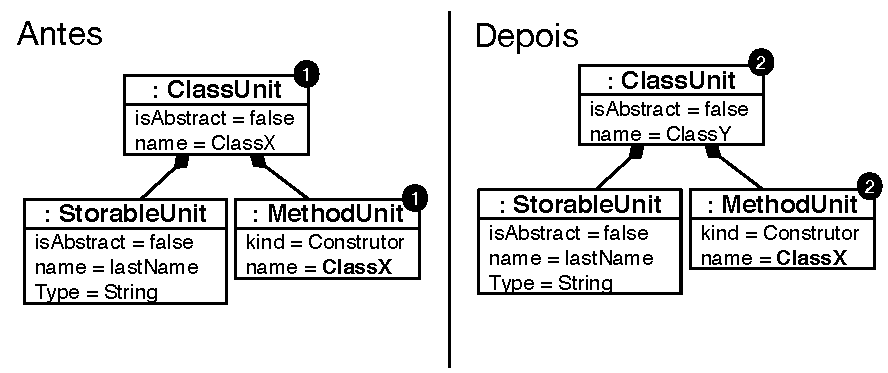
\includegraphics[scale=0.6]{images/antes_e_depois_rename_classUnit.pdf}
	\fautor
	\label{fig:antes_e_depois_rename_classUnit}
	\captionof{figure}{instância simplificada do KDM antes e depois da refatoração \textit{Rename ClassUnit} - parte 2}
	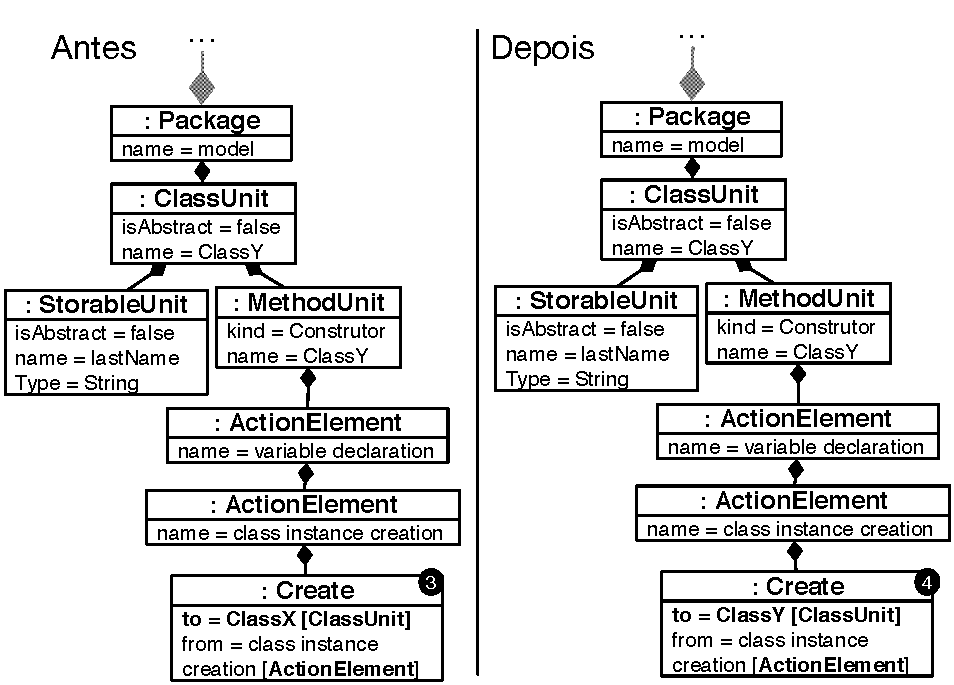
\includegraphics[scale=0.6]{images/antes_e_depois_rename_classUnit_Create.pdf}
	\fautor
	\label{fig:antes_e_depois_rename_classUnit_create}
\end{minipage}\hfill
			\item Algoritmo: 
			    \begin{itemize}
			        \item \{\texttt{ClassUnit}Selecionada\}.renameClassUnit(\{novoNome\});
			        \item para cada construtor - \texttt{MethodUnit.Kind=Construtor}.renameMethodUnit(\{novoNome\});
			        \item para cada referência da \{\texttt{ClassUnit}Selecionada\} deve-se mudar o meta-relacionamento \texttt{to} das metaclasses \texttt{Calls}, \texttt{Creates}, etc. 
			    \end{itemize}
		\end{enumerate}
	\item Especificação Formal:
		\begin{enumerate}
			\item Pré-condição: 
			\begin{codigo}[caption={[OCL representando a pré-condição da refatoração \textit{Rename ClassUnit}.] Pré-condição da refatoração \textit{Rename ClassUnit}.},escapeinside={(*@}{@*)}, basicstyle=\footnotesize, label={codigo:pre_renameClassUnit}, language=OCL]{Name}
context ClassUnit::preRenameClassUnit(newName: String)
pre : newName.isValidadName() 
and not ClassUnit.eContainer.codeElement(*@$\rightarrow$@*)exist (c : ClassUnit | c.name = newName) 
and not ClassUnit.codeElement(*@$\rightarrow$@*)exist (m: MethodUnit | m.name = newName and m.kind =  method)
\end{codigo}

%É importante observar que deve-se especificar a \texttt{ClassUnit} que será renomeada, bem como definir o novo nome dessa \texttt{ClassUnit} antes de executar a pré-condição, como apresentado no Código-fonte~\ref{codigo:pre_renameClassUnit}. 
Na linha 1 do Código-fonte~\ref{codigo:pre_renameClassUnit} é declarado o nome da pré-condição, também é declarado que essa restrição, é apenas executada para instâncias da metaclasse \texttt{ClassUnit}. Na linha 2 verifica-se se o parâmetro \texttt{newName} é um nome válido. Posteriormente, na linha 3 é verificado também se existe outra instância de \texttt{ClassUnit} com o mesmo valor do parâmetro \texttt{newName}. Linha 4 é verificado se existe alguma instância de \texttt{MethodUnit} com o mesmo valor do parâmetro \texttt{newName}. Caso a restrição definida na pré-condição seja válida a refatoração \textit{Rename ClassUnit} é executada.
			\item Algoritmo: 
	\begin{codigo}[caption={[ATL representando a refatoração \textit{Rename ClassUnit}.] ATL da refatoração \textit{Rename ClassUnit}.},escapeinside={(*@}{@*)}, basicstyle=\footnotesize, label={codigo:rename_classUnit_refatoracao}, language=ATL]{Name}
module renameClassUnit;
create OUT : MM refining IN : MM;
rule renameClassUnit {
	from
		source : MM!ClassUnit (source.name = (*@\aspas{\{\texttt{ClassUnit}Selecionada\}}@*))
	to 
		target : MM!ClassUnit (
			name (*@$\leftarrow$@*) (*@\aspas{newName}@*)
		)
}
rule renameConstrutor {
	from
		source : MM!MethodUnit (source.name = (*@\aspas{\{\texttt{ClassUnit}Selecionada\}}@*) and source.kind=(*@\aspas{constructor}@*))
	to 
		target : MM!MethodUnit (
			name (*@$\leftarrow$@*) (*@\aspas{newName}@*)
		)
}
\end{codigo}
			Como pode ser observado no Código-fonte~\ref{codigo:rename_classUnit_refatoracao} na linha 1 primeiramente é definido o nome da refatoração. Em seguida, na linha 2 é apresentado o cabeçalho da refatoração, note a palavra-chave \textit{refining}. Essa palavra-chave informa que essa transformação/refatoração é do tipo endógenas (\textit{in-place}) (ver Capítulo~\ref{chapter:fundamentacao_teorica} Seção~\ref{sec:transformacoes_de_modelos}), ou seja, irá alterar uma mesma instância do metamodelo KDM. Linha 3 até linha 10 a primeira regra é definida. Linha 5 uma condição de guarda é definida, a qual informa que apenas uma instância da metaclasse do tipo \texttt{ClassUnit} que possui um nome especifico será selecionada para a refatoração. Nas linhas 7, 8 e 9 o nome da instância da metaclasse do tipo \texttt{ClassUnit} é alterado. Posteriormente deve-se também alterar o nome do construtor, isso é realizado na regra especificado nas linha 11 até 17. Na linha 13 uma condição de guarda é especificada para informar que apenas métodos do tipo construtor devem ser obtidos, bem como o método deve possuir o mesmo nome da classe selecionada para aplicar a refatoração. Linhas 15, 16 e 17 o nome do construtor é alterado. Observe que tanto \{\texttt{ClassUnit}Selecionada\} quanto \{\textit{newName}\} são parâmetros que devem ser especificados pelo engenheiro. Assim, foi criado um \textit{plug-in} para auxiliar o engenheiro durante a especificação e execução das refatorações. Maiores informações sobre esse \textit{plug-in} estão no Capítulo X.     
			\item Pós-condição:
			 \begin{codigo}[caption={[OCL representando a pós-condição da refatoração \textit{Rename ClassUnit}.] Pós-condição da refatoração \textit{Rename ClassUnit}.},escapeinside={(*@}{@*)}, basicstyle=\footnotesize, label={codigo:pos_condicao_rename_classUnit}, language=OCL]{Name}
 context ClassUnit::RenameClassUnit(newName: String)
 post : name = newName and ClassUnit.eContainer.codeElement(*@$\rightarrow$@*)exist (m : MethodUnit | implies m.name = newName)
\end{codigo}
Na linha 1 do Código-fonte~\ref{codigo:pos_condicao_rename_classUnit} é declarado o nome da pós-condição, também é declarado que essa restrição, é apenas executada para o contexto de instâncias da metaclasse \texttt{ClassUnit}. Na linha 2 o parâmetro \texttt{newName} é comparado com o nome da \texttt{ClassUnit} refatorada, além disso, na linha 2 também é verificado se o construtor também foi alterado o seu nome corretamente. Se ambas as condições foram válidas, a refatoração foi realizada com sucesso.
		\end{enumerate}
\end{enumerate}
		
%--------------------------
\subsection{Refatoração \textit{Push Down StorableUnit}}
Nesta seção a refatoração \textit{Push Down StorableUnit} é apresentada. Essa refatoração é utilizada para remover a generalização de atributos, ou seja, um atributo é apenas utilizado em algumas sub-classes não em todas, assim, não é interessante manter a generalização do atributo na super-classe, uma vez que cada sub-classe pode definir um comportamento para o atributo~\cite{Fowler1999}.

\begin{enumerate}
	\item Especificação Informal:
		\begin{enumerate}
			\item Nome: \textit{Push Down StorableUnit};
			\item Definição:
			    \begin{itemize}
			        \item \texttt{StorableUnit}Selecionado - um atributo que será movido para sub-classes;
			        \item \texttt{ClassUnit} - uma classe na qual o \{\texttt{StorableUnit}Selecionado\} é definido;
			        \item sub-\texttt{ClassUnit}Selecionadas - sub-classes de \{\texttt{ClassUnit}\}.
			    \end{itemize}
			\item Objetivo: Mover um \{\texttt{StorableUnit}Selecionado\} para as \{sub-\texttt{ClassUnit}Selecionadas\}.
			\item Descrição (opcional): \{\texttt{StorableUnit}Selecionado\} é utilizada em apenas algumas sub-classes.
			\item Pré-condição:
			    \begin{itemize}
			        \item \{\texttt{StorableUnit}Selecionado\} não é utilizado em \texttt{ClassUnit};
			        \item as sub-\texttt{ClassUnit}Selecionadas não contêm as mesmas características do \{\texttt{StorableUnit} Selecionado\}, ou seja, os nomes e tipos são diferentes.
			    \end{itemize}
			\item Pós-condição:
			    \begin{itemize}
			        \item \{\texttt{StorableUnit}Selecionado\} não é definido em \texttt{ClassUnit};
			        \item todos os \textit{siblings} de \{\texttt{StorableUnit}Selecionado\} estão definidos nas sub-\texttt{ClassUnit}Selecionadas.
			    \end{itemize}
			\item Mecanismo: Na Figura~\ref{fig:antes_e_depois_pushDown_StorableUnit} duas instâncias simplificada do KDM são ilustradas, a parte superior ilustra a instância antes da realização da refatoração \textit{Push Down StorableUnit} e a parte inferior representa o resultado da refatoração. Como observado, o primeiro passo da refatoração \textit{Push Down StorableUnit} é selecionar um específico \texttt{StorableUnit}, Figura~\ref{fig:antes_e_depois_pushDown_StorableUnit} \ding{202}. Em seguida, deve-se selecionar as sub-classes que realmente utilizam esse \texttt{StorableUnit} para move-lo, com ilustrado na Figura~\ref{fig:antes_e_depois_pushDown_StorableUnit} \ding{203}. Posteriormente o \{\texttt{StorableUnit}Selecionado\} é movido para as sub-\texttt{ClassUnit}Selecionadas, como ilustrado na parte inferior da Figura~\ref{fig:antes_e_depois_pushDown_StorableUnit} \ding{205}. Note que a instância da \texttt{ClassUnit} que havia o \{\texttt{StorableUnit}Selecionado\} não possui mais sua instância, como apresentado na Figura~\ref{fig:antes_e_depois_pushDown_StorableUnit} \ding{204}.
			
			
\begin{minipage}{.90\textwidth}
	\vspace*{\fill}
  \centering
	% Requires \usepackage{graphicx}
	\captionof{figure}{Instância simplificada do KDM antes e depois da refatoração \textit{Push Down StorableUnit}}
	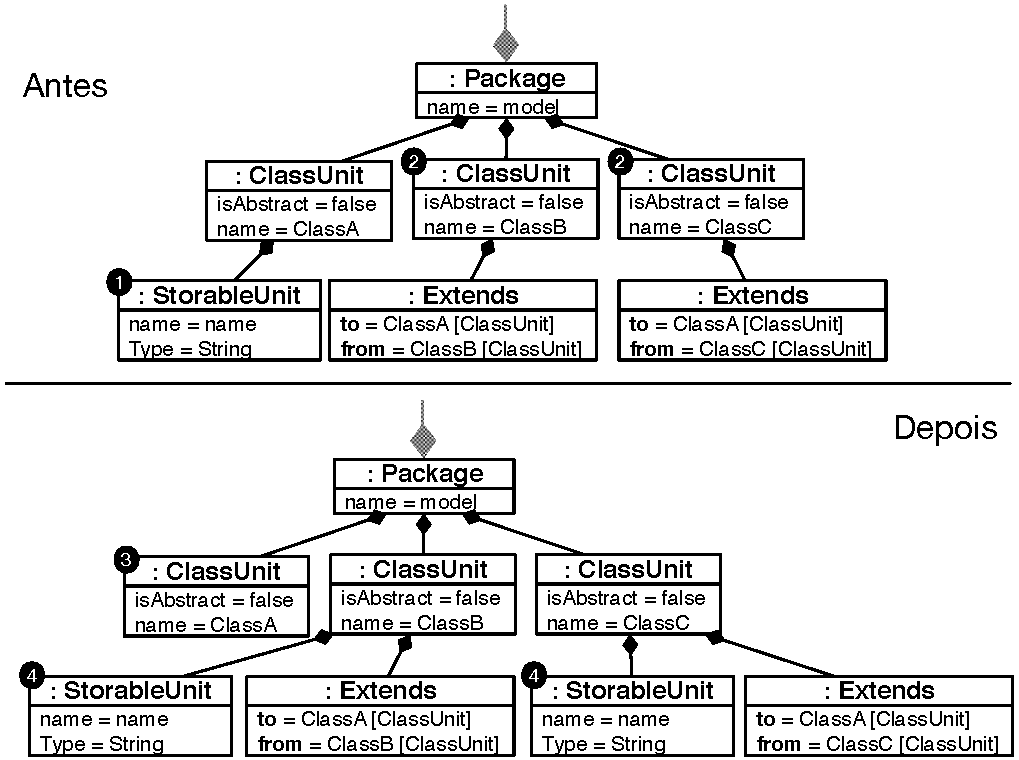
\includegraphics[scale=0.6]{images/antes_e_depois_push_down_storableUnit.pdf}
	\fautor
	\label{fig:antes_e_depois_pushDown_StorableUnit}
\end{minipage}\hfill
			\item Algoritmo: 
			    \begin{itemize}
			        \item para cada sub-\texttt{ClassUnit}Selecionadas que realmente usa o \{\texttt{StorableUnit}Selecionado\} - sub-\texttt{ClassUnit}Selecionadas.add(\{\texttt{StorableUnit}Selecionado\})
			        \item \{\texttt{ClassUnit}\}.remove(\{\texttt{StorableUnit}Selecionado\}). 
			    \end{itemize} 
	    \end{enumerate}
		\item Especificação Formal:
		\begin{enumerate}
			\item Pré-condição: 
			\begin{codigo}[caption={[OCL representando a pré-condição da refatoração \textit{Push Down StorableUnit}.] Pré-condição da refatoração \textit{Push Down StorableUnit}.},escapeinside={(*@}{@*)}, basicstyle=\footnotesize, label={codigo:pre_push_down_storableUnit}, language=OCL]{Name}
context StorableUnit::PushDownStorableUnit(subClasses:(ClassUnit))
pre : self.refImmediateComposite().codeElement(*@$\rightarrow$@*)forAll (m: MethodUnit |  not (m.codeRelation(*@$\rightarrow$@*)exists(r: Reads | r.to = self)) 
and not (m.codeRelation(*@$\rightarrow$@*)exists (w:Writes | w.to = self)) 
and not (m.codeRelation(*@$\rightarrow$@*)exists (a: Addresses | a.to = self) 
and subClasses(*@$\rightarrow$@*)forAll (c: ClassUnit | not c.codeElement(*@$\rightarrow$@*)exists(s: StorableUnit | s.name = self.name)))
\end{codigo}



%É importante observar que deve-se especificar a \texttt{ClassUnit} que será renomeada, bem como definir o novo nome dessa \texttt{ClassUnit} antes de executar a pré-condição, como apresentado no Código-fonte~\ref{codigo:pre_renameClassUnit}. 
Na linha 1 do Código-fonte~\ref{codigo:pre_push_down_storableUnit} é declarado a assinatura da pré-condição da refatoração \textit{Push Down StorableUnit}. Note que apenas é utilizado como parâmetro as sub-classes selecionadas para mover o \{\texttt{StorableUnit}Selecionado\}. Na linha 2 a instância da \texttt{ClassUnit} que contêm o \{\texttt{StorableUnit}Selecionado\} é obtida por meio da função \texttt{refImmediateComposite()}. Posteriormente, todas as instâncias de \texttt{MethodUnit} são obtidas para realizar uma iteração. Ainda na linha 2, essa iteração verifica se o \{\texttt{StorableUnit}Selecionado\} é lido em alguma instância de \texttt{MethodUnit}. Similarmente, na linha 3 e 4 todos os \texttt{MethodUnits} são verificados para identificar se o \{\texttt{StorableUnit}Selecionado\} é escrito e utilizado. Na linha 5 todas as \{sub-\texttt{ClassUnit}Selecionadas\} são verificadas para identificar se existe uma instância similar ao \{\texttt{StorableUnit}Selecionado\} antes de realizar a refatoração. Caso a pré-condição definida seja válida a refatoração \textit{Push Down StorableUnit} é executada.
			\item Algoritmo: 
	\begin{codigo}[caption={[ATL representando a refatoração \textit{Push Down StorableUnit}.] ATL da refatoração \textit{Push Down StorableUnit}.},escapeinside={(*@}{@*)}, basicstyle=\footnotesize, label={codigo:push_Down_StorableUnit_ATL}, language=ATL]{Name}
module pushDownStorableUnit;
create OUT : MM refining IN : MM;
rule pushDownStorableUnit {
	from
		source : MM!ClassUnit (source.name = (*@\aspas{\{sub-\texttt{ClassUnit}Selecionada\}}@*) or source.name = (*@\aspas{\{sub-\texttt{ClassUnit}Selecionada\}}@*))
	to 
		target : MM!ClassUnit (
			codeElement(*@$\leftarrow$@*)source.codeElement(*@$\rightarrow$@*)including(attr)
		),
		attr: MM!StorableUnit (
			name(*@$\leftarrow$@*)(*@\{\texttt{StorableUnit}Selecionado.name\}@*),
			type(*@$\leftarrow$@*)(*@\{\texttt{StorableUnit}Selecionado.type\}@*)
		)
}
rule removeStorableUnitFromSuperClass {
	from
		source : MM!StorableUnit (source.name = (*@\{\texttt{StorableUnit}Selecionado.name\}@*) and not source.refImmediateComposite().codeRelation.isEmpty())
	to
		drop
}
\end{codigo}
Na linha 1 do Código-fonte~\ref{codigo:push_Down_StorableUnit_ATL} o nome da refatoração é definido. Em seguida, na linha 2 é apresentado o cabeçalho da refatoração, novamente a palavra-chave \textit{refining} é especificada para informar que a transformação/refatoração é do tipo endógenas (ver Capítulo~\ref{chapter:fundamentacao_teorica} Seção~\ref{sec:transformacoes_de_modelos}). Posteriormente, nas linhas 3 até 13 a primeira regra dessa refatoração é definida. Na linha 5 uma condição de guarda é definida para identificar quais são as \{sub-\texttt{ClassUnit}Selecionadas\}. Em seguida, linhas 7, 8 e 9 informa que uma nova instância de \texttt{StorableUnit} será criado nas \{sub-\texttt{ClassUnit}Selecionadas\}. Nas linhas 10, 11 e 12 os meta-atributos do \{\texttt{StorableUnit}Selecionado\} são copiados. Após mover o \{\texttt{StorableUnit}Selecionado\} para as sub-classes, o próximo passo é remover o \{\texttt{StorableUnit}Selecionado\} da super-classe. Esse passo é representado na regra descrita nas linhas 15 até 20. Na linha 17 o \{\texttt{StorableUnit}Selecionado\} é identificado, depois na linha 19 a palavra-chave \textit{drop} é utilizada, a qual especifica que uma determinada instância será removida, neste caso o \{\texttt{StorableUnit}Selecionado\}.   
			\item Pós-condição:
			 \begin{codigo}[caption={[OCL representando a pós-condição da refatoração \textit{Push Down StorableUnit}.] Pós-condição da refatoração \textit{Push Down StorableUnit}.},escapeinside={(*@}{@*)}, basicstyle=\footnotesize, label={codigo:pos_condicao_pushDown_StorableUnit}, language=OCL]{Name}
context StorableUnit::PushDownStorableUnit(subClasses:Bag(ClassUnit))
post : self.refImmediateComposite().codeElement(*@$\rightarrow$@*)exists (s: StorableUnit | not (s.name = self.name)) 
and subClasses->forAll (c: ClassUnit | c.codeElement(*@$\rightarrow$@*)exists (s: StorableUnit | s.name = self.name and s.type = self.type))
\end{codigo}
Na linha 1 do Código-fonte~\ref{codigo:pos_condicao_pushDown_StorableUnit} é declarado o nome da pós-condição. Na linha 2 é verificado se o \{\texttt{StorableUnit}Selecionado\} ainda está na super-classe. Posteriormente, na linha 3, para todas as \{sub-\texttt{ClassUnit}Selecionadas\} são verificadas para garantir que o \{\texttt{StorableUnit}Selecionado\} foi adicionado corretamente. Caso afirmativo a refatoração foi realizada com sucesso.
		\end{enumerate}
	\end{enumerate}		
	
	
	
%--------------------------
\subsection{Refatoração \textit{Extract ClassUnit}}
Nesta seção a refatoração \textit{Extract ClassUnit} é apresentada. Essa refatoração é utilizada quando uma determinada classe está fazendo o trabalho que deveria ser realizada por duas classes~\cite{Fowler1999}. 

\begin{enumerate}
	\item Especificação Informal:
		\begin{enumerate}
			\item Nome: \textit{Extract ClassUnit};
			\item Definição:
			    \begin{itemize}
			        \item \texttt{ClassUnit}Selecionada - a classe que contêm os atributos e métodos que devem ser movido para a nova classe;
			        \item novoNome - um novo nome para a nova classe a ser criada;
			        \item \texttt{StorableUnit}Selecionados - atributos relevantes selecionados para serem movido para a nova classe;
			        \item \texttt{MethodUnit}Selecionados - métodos relevantes selecionados para serem movidos para a nova classe.
			    \end{itemize}
			\item Objetivo: Criar uma nova \texttt{ClassUnit} e mover os \texttt{StorableUnit}Selecionados e \texttt{MethodUnit}Selecionados para esse nova instância.
			\item Descrição (opcional): \texttt{ClassUnit}Selecionada está realizando o trabalho que deveria ser realizado por duas classes.
			\item Pré-condição:
			    \begin{itemize}
			        \item \{\texttt{ClassUnit}Selecionada\} deve contêm atributos e métodos para mover para a nova classe;
			        \item os \{\texttt{StorableUnit}Selecionados\} não são utilizados na \{\texttt{ClassUnit}Selecionada\};
			        \item os \{\texttt{MethodUnit}Selecionados\} não são utilizados na \{\texttt{ClassUnit}Selecionada\};
			        \item o \{novoNome\} da nova instância da \texttt{ClassUnit} deve seguir as convenções válidas para nomes de classes;
			        \item não deve existir outra instância da \texttt{ClassUnit} com o mesmo nome dentro do mesmo \texttt{Package}.
			    \end{itemize}
			\item Pós-condição:
			    \begin{itemize}
			        \item \{\texttt{StorableUnit}Selecionados\} não são definido em \{\texttt{ClassUnit}Selecionada\};
			        \item \{\texttt{MethodUnit}Selecionados\} não são definido em \{\texttt{ClassUnit}Selecionada\};
			        \item todos os \{\texttt{StorableUnit}Selecionados\} e \{\texttt{MethodUnit}Selecionados\} estão definidos na nova instância da \texttt{ClassUnit} criada.
			    \end{itemize}
			\item Mecanismo: O primeiro passo da refatoração \textit{Extract ClassUnit} é selecionar um conjunto de \texttt{StorableUnits} e/ou \texttt{MethodUnits} que serão movidos para uma nova instância de metaclasse \texttt{ClassUnit}, no exemplo ilustrado na Figura~\ref{fig:antes_e_depois_extract_ClassUnit} \ding{202} duas instâncias de \texttt{StorableUnits} são selecionadas. Posteriormente, uma nova instância da metaclasse \texttt{ClassUnit} é criada e adicionada o mesmo \texttt{Package} que a instância da metaclasse \texttt{ClassUnit} que contêm os \{\texttt{StorableUnit}Selecionados\}, como ilustrado na Figura~\ref{fig:antes_e_depois_extract_ClassUnit} \ding{204}. Em seguida, os todos os \{\texttt{StorableUnit}Selecionados\} são movidos para esse nova instância, como representado na Figura~\ref{fig:antes_e_depois_extract_ClassUnit} \ding{203}. Ainda na Figura~\ref{fig:antes_e_depois_extract_ClassUnit} \ding{205} é possível observar que uma outra metaclasse denominada \texttt{HasType} foi também instanciada. Essa metaclasse ilustra o relacionamento de associação entre duas classes no metamodelo KDM. Note que igual similar a metaclasse \texttt{Extends} e \texttt{Implements}, a metaclasse \texttt{HasType} possui duas meta-relacionamentos, \texttt{to} e \texttt{from}.
\begin{minipage}{.90\textwidth}
	\vspace*{\fill}
  \centering
	% Requires \usepackage{graphicx}
	\captionof{figure}{Instância simplificada do KDM antes e depois da refatoração \textit{Extract ClassUnit}}
	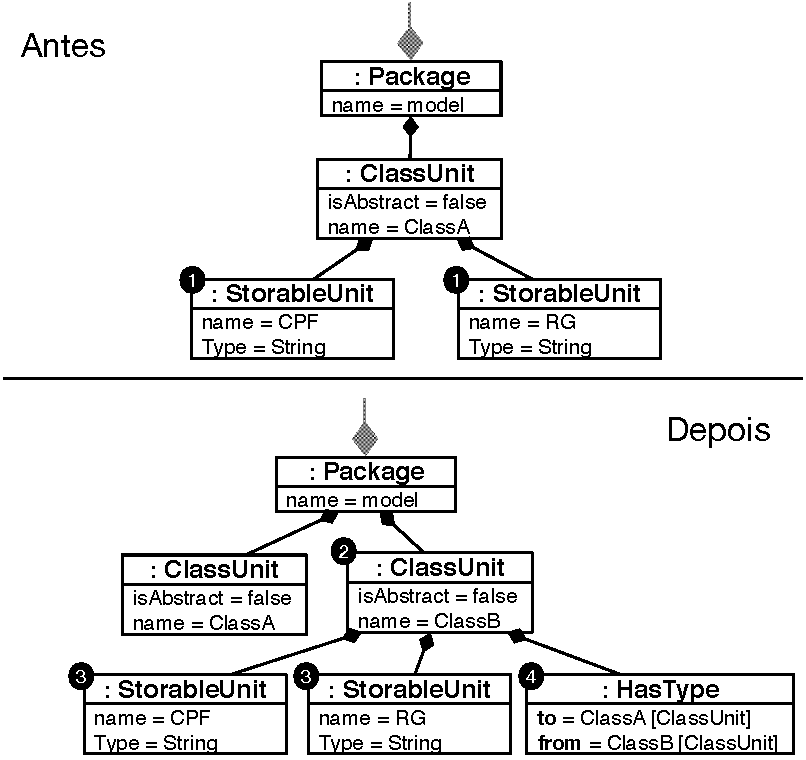
\includegraphics[scale=0.6]{images/antes_e_depois_refatoracao_extract_ClassUnit.pdf}
	\fautor
	\label{fig:antes_e_depois_extract_ClassUnit}
\end{minipage}\hfill
			\item Algoritmo: 
			    \begin{itemize}
			        \item createNewClassUnit(\{novoNome\});
			        \item adiciona essa nova instância dentro de um \texttt{Package};
			        \item para cada \{\texttt{StorableUnit}Selecionado\} - move(\{newClassUnit\}, \{\texttt{StorableUnit}Selecionado\})
			        \item para cada \{\texttt{MethodUnit}Selecionado\} - move(\{newClassUnit\}, \{\texttt{MethodUnit}Selecionado\});
			        \item createNewHasType(\{newClassUnit\}, \{\texttt{ClassUnit}Selecionada\}).
			    \end{itemize} 
	    \end{enumerate}
		\item Especificação Formal:
		\begin{enumerate}
			\item Pré-condição: 
			\begin{codigo}[caption={[OCL representando a pré-condição da refatoração \textit{Extract ClassUnit}.] Pré-condição da refatoração \textit{Extract ClassUnit}.},escapeinside={(*@}{@*)}, basicstyle=\footnotesize, label={codigo:pre_extract_ClassUnit}, language=OCL]{Name}
context ClassUnit::ExtractClassUnit(newName: String, storableUnitSelected:(StorableUnit), methodUnitSelected: (MethodUnit))
pre : newName.isValidName() and not self.refImmediateComposite().codeElement(*@$\rightarrow$@*)exist (c: ClassUnit | c.name = newName) 
and not storableUnitSelected(*@$\rightarrow$@*)forAll (s: StorableUnit | self.codeElement(*@$\rightarrow$@*)forAll (m: MethodUnit | not (m.codeRelation(*@$\rightarrow$@*)exists(re: Reads | re.to = s)) and not (m.codeRelation(*@$\rightarrow$@*)exists (wr:Writes | wr.to = s)) and not (m.codeRelation(*@$\rightarrow$@*)exists (add: Addresses | add.to = s)) 
and not methodUnitSelected(*@$\rightarrow$@*)forAll (m: MethodUnit | self.codeElement(*@$\rightarrow$@*)forAll (m: MethodUnit | not (m.codeRelation(*@$\rightarrow$@*)exists (call: Calls| call.to = m)))))
\end{codigo}
%É importante observar que deve-se especificar a \texttt{ClassUnit} que será renomeada, bem como definir o novo nome dessa \texttt{ClassUnit} antes de executar a pré-condição, como apresentado no Código-fonte~\ref{codigo:pre_renameClassUnit}. 
Na linha 1 do Código-fonte~\ref{codigo:pre_extract_ClassUnit} é declarado a assinatura da pré-condição da refatoração \textit{Extract ClassUnit}, note que essa pré-condição possui três parâmetros: o nome da nova instância da metaclasse \texttt{ClassUnit}, um conjunto de \{\texttt{StorableUnit}Selecionado\} e um conjunto de \{\texttt{MethodUnit}Selecionado\}. Na linha 2 é verificado se o parâmetro \{newName\} é válido para ser utilizado como nome de classe. Ainda na linha 2 a instância de da metaclasse \texttt{Package} é obtida por meio da função \texttt{refImmediateComposite()} para verificar dentro do escopo deste pacote se não existe nenhuma classe com o mesmo nome. Na linha 3 para cada \{\texttt{StorableUnit}Selecionado\} é verificado se são utilizados dentro de uma instância de \texttt{MethodUnit}, ou seja, verifica-se se o \{\texttt{StorableUnit}Selecionado\} é escrito e utilizado nos métodos. Similarmente, na linha 4 é verificado para cada \{\texttt{MethodUnit}Selecionado\} se o mesmo é chamado em algum lugar. Caso a pré-condição definida seja válida a refatoração \textit{Extract ClassUnit} é executada.
			\item Algoritmo: 
	\begin{codigo}[caption={[ATL representando a refatoração \textit{Extract ClassUnit}.] ATL da refatoração \textit{Extract ClassUnit}.},escapeinside={(*@}{@*)}, basicstyle=\footnotesize, label={codigo:extract_classUnit_ATL}, language=ATL]{Name}
module createAnClassThenMoveAnAttribute;
create OUT : MM refining IN : MM;
rule extractClassUnit {
	from
		source : MM!Package (source.name = (*@\aspas{\{\texttt{ClassUnit}Selecionada.refImmediateComposite()\}}@*))
	to 
		target: MM!Package (
			codeElement(*@$\leftarrow$@*)source.codeElement(*@$\rightarrow$@*)including(newClassUnit)
		),
		newClassUnit: MM!ClassUnit (
			name(*@$\leftarrow$@*)(*@\aspas{\{newName\}}@*),
			codeElement(*@$\leftarrow$@*)thisModule.getMethodUnits(thisModule.getClassUnit((*@\aspas{\{\texttt{ClassUnit}Selecionada\}}@*)), (*@\aspas{\{\texttt{MethodUnit}Selecionados\}}@*)),
			codeElement(*@$\leftarrow$@*)thisModule.getStorableUnits(thisModule.getClassUnit((*@\aspas{\{\texttt{ClassUnit}Selecionada\}}@*)), (*@\aspas{\{\texttt{StorableUnit}Selecionados\}}@*)))
rule createLinkExtractClassUnit {
	from
		source : MM!ClassUnit (source.name = (*@\aspas{\{\texttt{ClassUnit}Selecionada\}}@*))
	to 
		target: MM!ClassUnit (
			codeRelation(*@$\leftarrow$@*)source.codeRelation(*@$\rightarrow$@*)including(hasType)
		),
		hasType: MM!HasType (
			to(*@$\leftarrow$@*)(*@\aspas{\{\texttt{ClassUnit}Selecionada\}}@*),
			from(*@$\leftarrow$@*)(*@\aspas{\{new\texttt{ClassUnit}\}}@*)
		)
}}
helper def : getClassUnit (className : String) : MM!ClassUnit = MM!ClassUnit.allInstances()->any(e | e.name = className);
helper def : getStorableUnit (classUnitToGetTheStorableUnit: MM!ClassUnit, nameOfAtt: String) : MM!StorableUnit = classUnitToGetTheStorableUnit.codeElement(*@$\rightarrow$@*)any(e | e.name = nameOfAtt);		
helper def : getMethodUnits (classUnitToGet: MM!ClassUnit, nameMethod: String) : MM!MethodUnit = classUnitToGet.codeElement(*@$\rightarrow$@*)any(e | e.name.equalsIgnoreCase(nameMethod));
\end{codigo}
Na linha 1 do Código-fonte~\ref{codigo:extract_classUnit_ATL} o nome da refatoração é definido. Em seguida, na linha 2 é apresentado o cabeçalho da refatoração. Nas linhas 3 até 13 a primeira regra dessa refatoração é definida. Na linha 5 uma condição de guarda é definida para identificar a instância da metaclasse \texttt{Package} que a nova instância da metaclasse \texttt{ClassUnit} será adicionada. Em seguida, as linhas 7, 8 e 9 representam que uma nova instância de \texttt{StorableUnit} será criado dentro da instância do \texttt{Package} identificado. Nas linhas 10 e 11 uma nova instância da metaclasse \texttt{ClassUnit} é efetivamente criada. Posteriormente, nas linhas 12 e 13 os \{\texttt{StorableUnit}Selecionados\} e os \{\texttt{MethodUnit}Selecionados\} são movidos para a \texttt{ClassUnit} recém instanciada. Após mover os \{\texttt{StorableUnit}Selecionados\} e os \{\texttt{MethodUnits}Selecionados\} para a \texttt{ClassUnit} o próximo passo é criar uma associação entre as duas instâncias de \texttt{ClassUnit}. Esse passo é representado na regra descrita nas linhas 14 até 25. Na linha 17 a {\texttt{ClassUnit}Selecionada\} é identificada, depois as linhas 18, 19 e 20 sinalizam que uma instância da metaclasse \texttt{HasType} será criada. Finalmente, nas linhas 21 até 23 a instância da metaclasse \texttt{HasType} é criada. Mas especificadamente, nas linhas 22 e 23 seus relacionamentos \texttt{to} e \texttt{from} são definidos, os quais representam a associação entre a classe que continha os \{\texttt{StorableUnit}Selecionados\} e os \{\texttt{MethodUnits}Selecionados\} e a nova instância da metaclasse \texttt{ClassUnit}, respectivamente. Linhas 26, 27 e 28 os \textit{helpers} que são utilizadas nessa refatoração são definidos.   
			\item Pós-condição:
			 \begin{codigo}[caption={[OCL representando a pós-condição da refatoração \textit{Extract ClassUnit}.] Pós-condição da refatoração \textit{Extract ClassUnit}.},escapeinside={(*@}{@*)}, basicstyle=\footnotesize, label={codigo:pos_condicao_extract_ClassUnit}, language=OCL]{Name}
context ClassUnit::ExtractClassUnit(storableUnitSelected: (StorableUnit), methodUnitSelected: (MethodUnit), newClass: ClassUnit)
post : self.codeElement(*@$\rightarrow$@*)exists (s: StorableUnit | not (storableUnitSelected(*@$\rightarrow$@*)forAll (sUS: StorableUnit | sUS.name = s.name))) and self.codeElement(*@$\rightarrow$@*)exists (m: MethodUnit | not (methodUnitSelected(*@$\rightarrow$@*)forAll (mUS: MethodUnit | mUS.name = m.name))) 
and newClass.codeElement(*@$\rightarrow$@*)exist (s: StorableUnit | (storableUnitSelected(*@$\rightarrow$@*)forAll (sUS: StorableUnit | sUS.name = s.name))) and newClass.codeElement(*@$\rightarrow$@*)exists (m: MethodUnit | not (methodUnitSelected(*@$\rightarrow$@*)forAll (mUS: MethodUnit | mUS.name = m.name)))        \end{codigo}
Na linha 1 do Código-fonte~\ref{codigo:pos_condicao_extract_ClassUnit} é declarado o nome da pós-condição. Na linha 2 é verificado se todos os \{\texttt{StorableUnit}Selecionados\} e \{\texttt{MethodUnits}Selecionados\} não estão definidos na \{\texttt{ClassUnit}Selecionada\}. Posteriormente, na linha 3, é verificado se todos os \{\texttt{StorableUnit}Selecionados\} e \{\texttt{MethodUnits}Selecionados\} foram efetivamentes movidos para a nova instância da metaclasse \texttt{ClassUnit}. Caso afirmativo a refatoração foi realizada com sucesso.
		\end{enumerate}
\end{enumerate}
	
	
\section{Considerações Finais}

Neste capítulo foi apresentado uma adaptação das refatorações já conhecidas e definidas na literatura para o metamodelo KDM. Mais especificamente foram escolhidas algumas refatorações propostas por~\citeonline{Fowler1999} para serem adaptadas para o metamodelo KDM. Embora ~\citeonline{Fowler1999} tenha definido um catálogo de refatoração para ser utilizado em código-fonte, mais de 60\% das refatorações (44 de 72) são ilustradas e explicadas utilizando modelos, mais especificadamente diagramas de classes da UML. Esta observação fez com que tais refatorações fossem adaptadas para o metamodelo KDM. 

Antes de adaptar as refatorações propostas por~\citeonline{Fowler1999} para o metamodelo KDM, primeiramente foi necessário identificar as metaclasses do KDM que tivesse características similares aos conceitos do POO, bem como instruções comumente utilizadas em todas as linguagens de programação, tais como, ramificações, iterações, etc. Dessa forma, esse capítulo também apresentou um mapeamento entre os conceitos do POO e o metamodelo KDM. Acredita-se que modernizadores pouco familiarizado com o metamodelo KDM podem gastar menos tempo durante a criação de novas refatorações com a utilização deste mapeamento, assim, qualquer exemplo de refatoração pode ser facilmente adaptada para o metamodelo KDM. 

As refatoração adaptado para o metamodelo KDM consistem de duas principais especificações - uma especificação informal e uma especificação formal. Na especificação informal a ideologia básica por trás da reforação é expressada por meio de linguagem natural. A segunda especificação é responsável por representas as pré- e pós-condições, bem como a transformação/refatoração propriamente dita em linguagens executáveis - OCL e ATL foram utilizadas. Ambas especificações são úteis para o modernizador -a especificação informal é utilizada para facilitar a compreensão e o propósito da refatoração,enquanto que a especificação formal facilita a implementação da refatoração. Além disso, a especificação formal é de extrema importância para facilitar a automação das refatorações. É importante destacar que neste capítulo apenas as refatorações \textit{Rename ClassUnit}, \textit{Pull Up StorableUnit}, \textit{Push Down StorableUnit} e \textit{Extract ClassUnit} são apresentadas e detalhadas.

No Capítulo~\ref{chapter:Toward_a_Refactoring_Metamodel_for_KDM} é apresentado um metamodelo para auxiliar o engenheiro a promover o reuso de refatorações no contexto do metamodelo KDM. Com a utilização desse metamodelo, informações (metadados) sobre refatorações podem ser reutilizadas de forma independente de linguagem e plataforma. No Capítulo~\ref{chapter:Abordagem_de_sincronizacao} uma abordagem para manter instâncias do metamodelo KDM sincronizada e consiste após a aplicação de refatoração é apresentada. No Capítulo~\ref{chapter:ferramenta_kdm_re} é apresentado uma ferramenta que foi desenvolvida dentro do ambiente Eclipse para apoiar o uso do catálogo de refatoração adaptado para o metamodelo KDM, dessa forma, essa ferramenta permite que modernizadores apliquem refatorações diretamente no metamodelo KDM. 
